\chapter{RRTFunnel}

\section{Funnel}

\subsection{Funnel library}

\subsection{Creating suitable funnels}

The funnels

\subsection{Nominal trajectories}

Generating the nominal trajectories is done through the \textit{Direct
  Collocation method}, as shown in \cite{DirectCollocation paper}.

\subsubsection{Richness of the funnel library}

Currently we only have three motion primitives in our motion libray. One left
motion, one straight, and one right, which is the symmetrical opposite of the
left motion. 

\section{Uncertainty}

\subsection{Effects of degree of uncertainty}

The RRTFunnel algorithm relies upon a set of precomputed funnels which have some
uncertainty robustness already built in, although the uncertainty has to be bounded.

\section{Distance metric}

\subsection{Euclidean distance metric}

The simplest mestric used is the euclidean distance metric. Here both the
closest node in the tree, and the local extension function use the euclidean
distance metric, which shows some significant shortfalls. As an example:

\begin{figure}
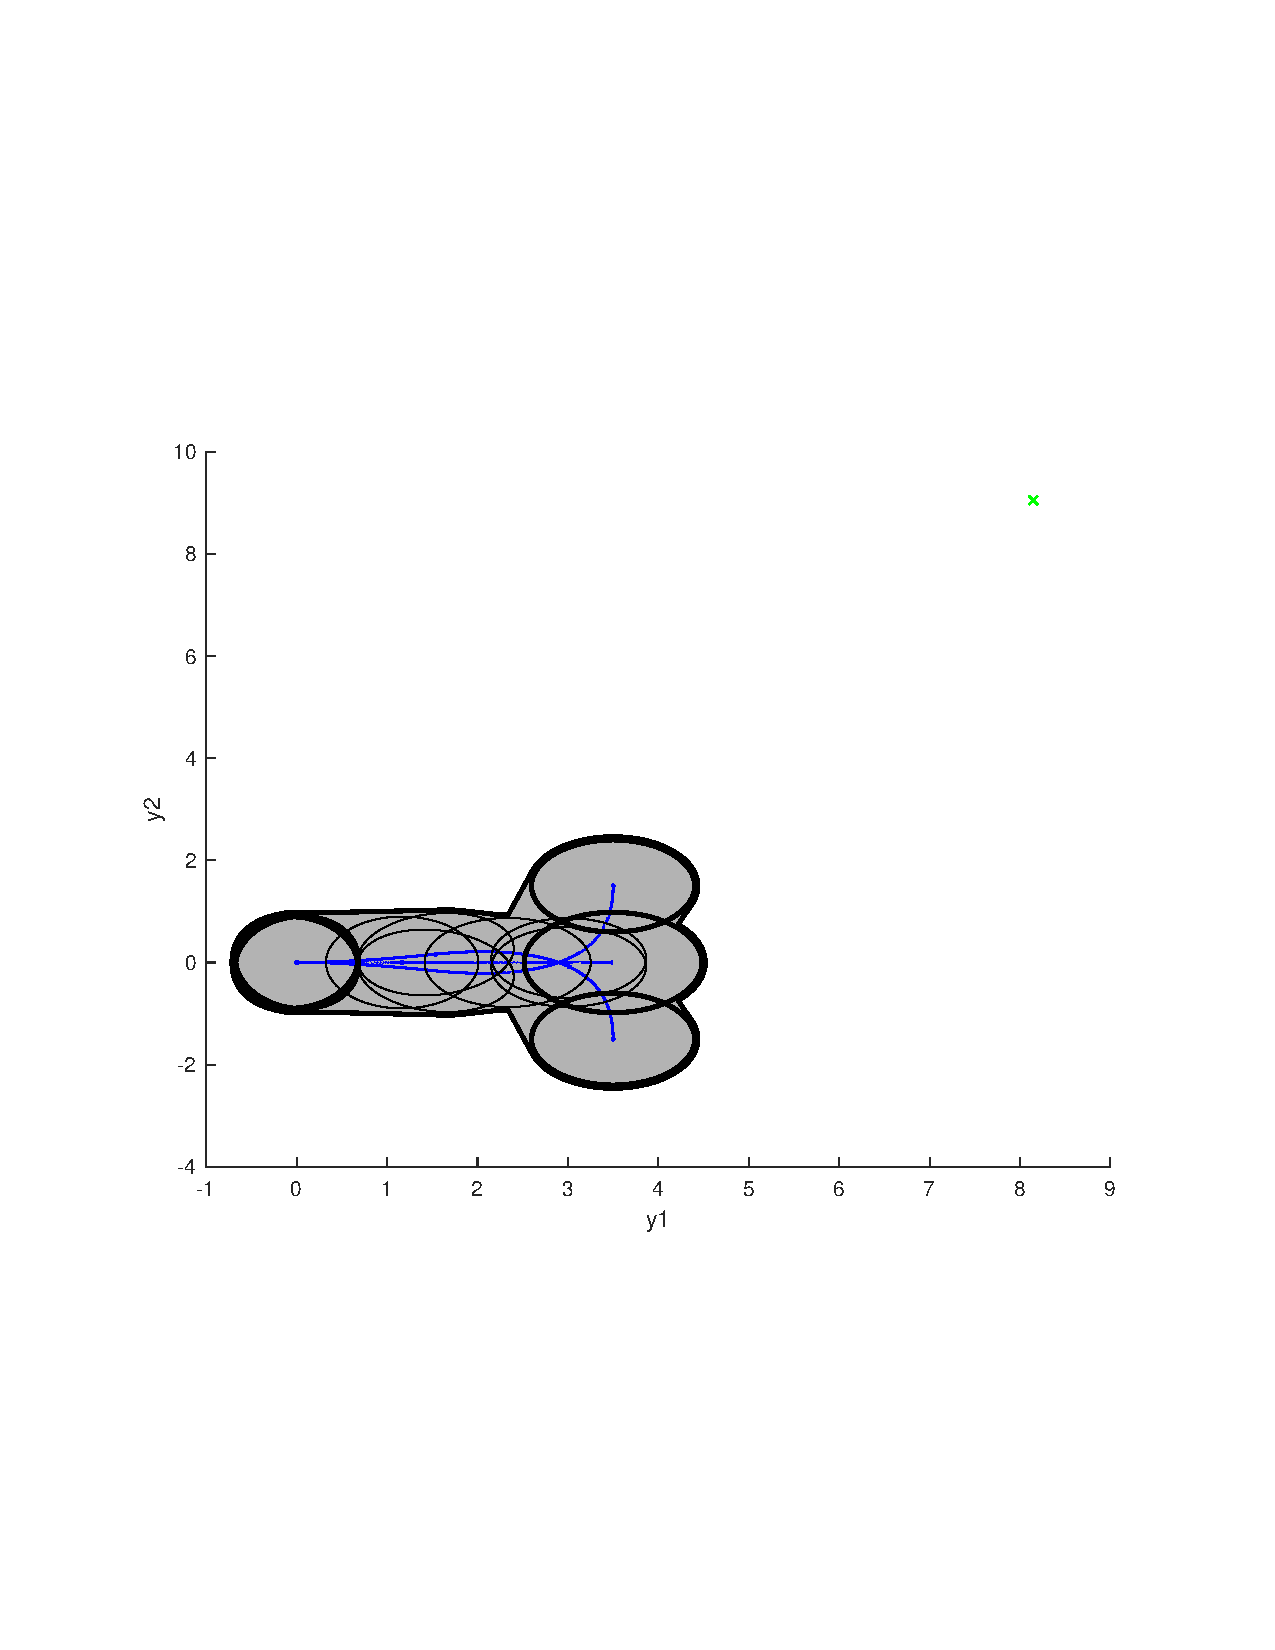
\includegraphics[scale=.5]{figures/rrtfunnel/euclidean-distance-closest-funnel1}
\caption{The three funnels in our motion primitive library, and a point in the
  state space,  selected at random, uniformly, from the interval \([0,10]\), and
  then projected down into the xy-plane.}
\end{figure}

\begin{figure}
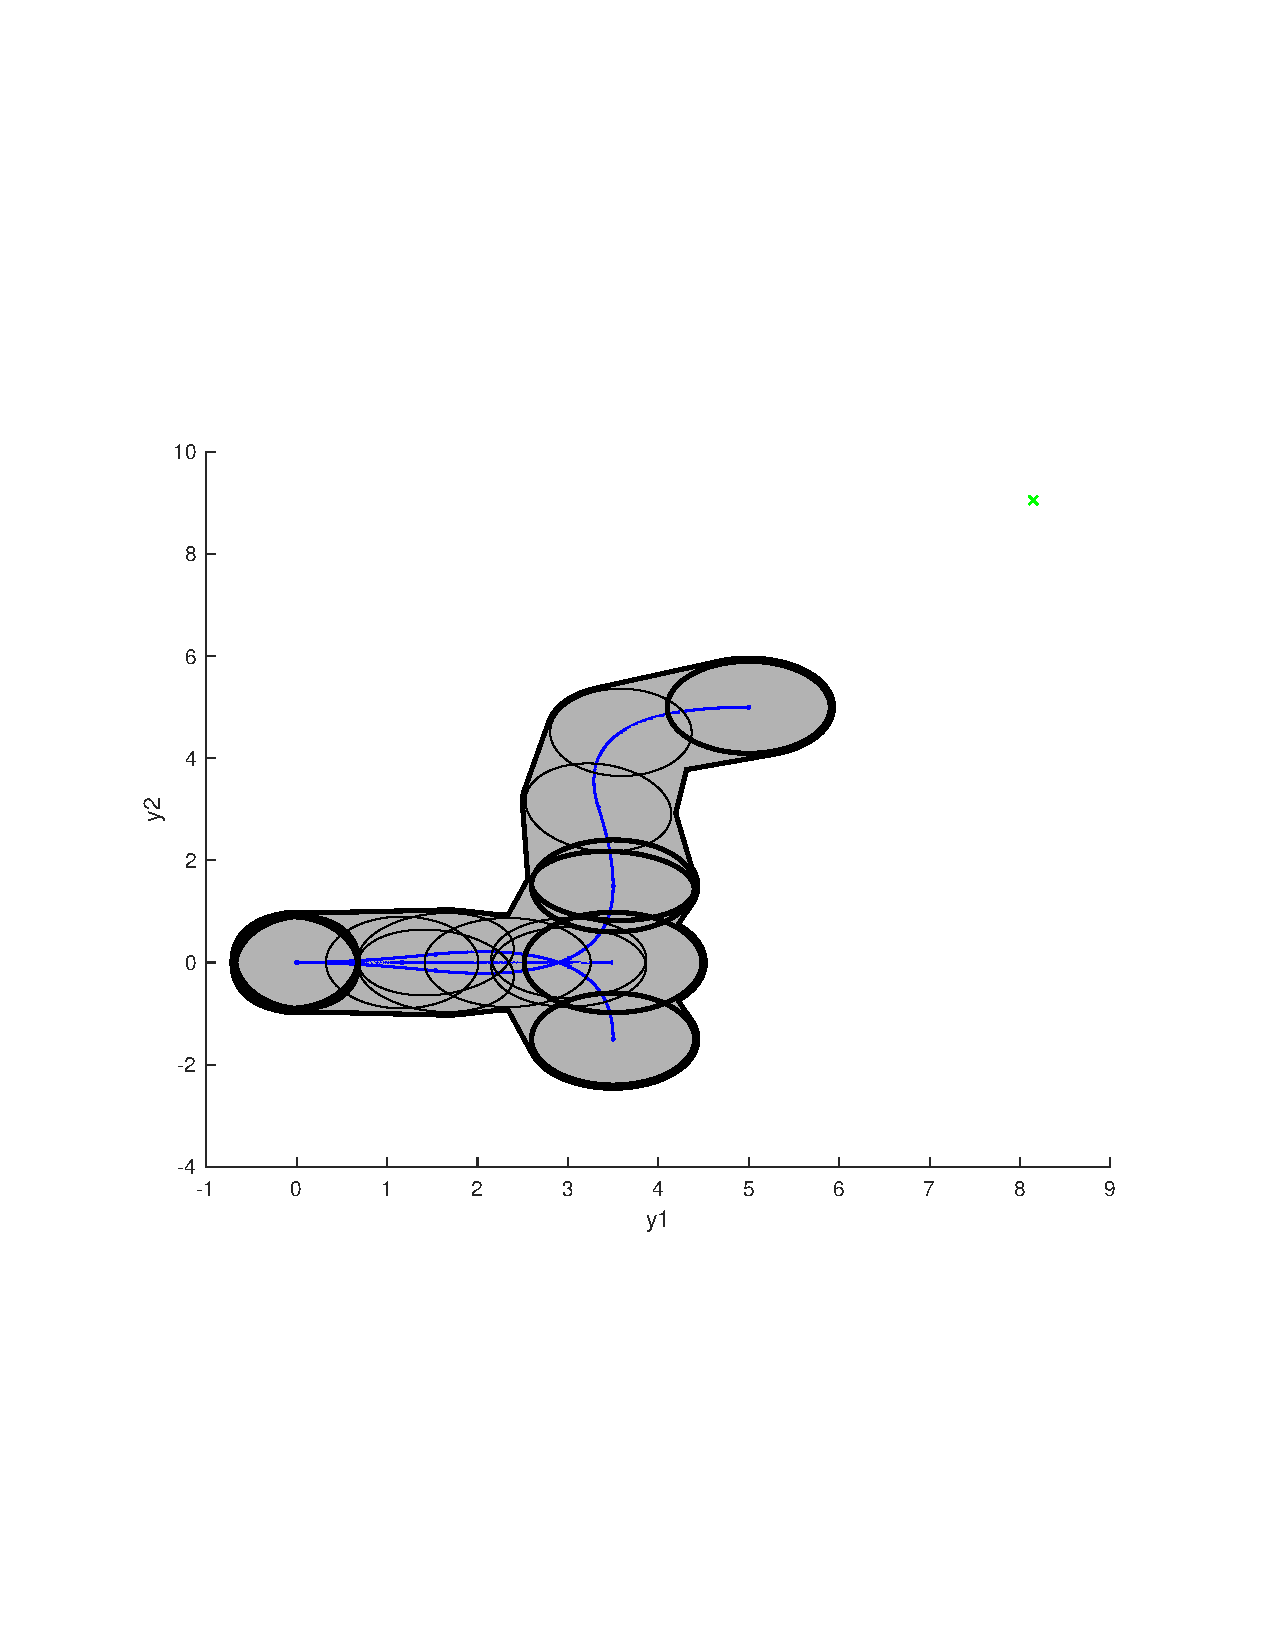
\includegraphics[scale=.5]{figures/rrtfunnel/euclidean-distance-closest-funnel2}
\caption{Tree expanded towards the point, again using the Euclidean norm as the
  metric for the local extension operator.}
\end{figure}

\begin{figure}
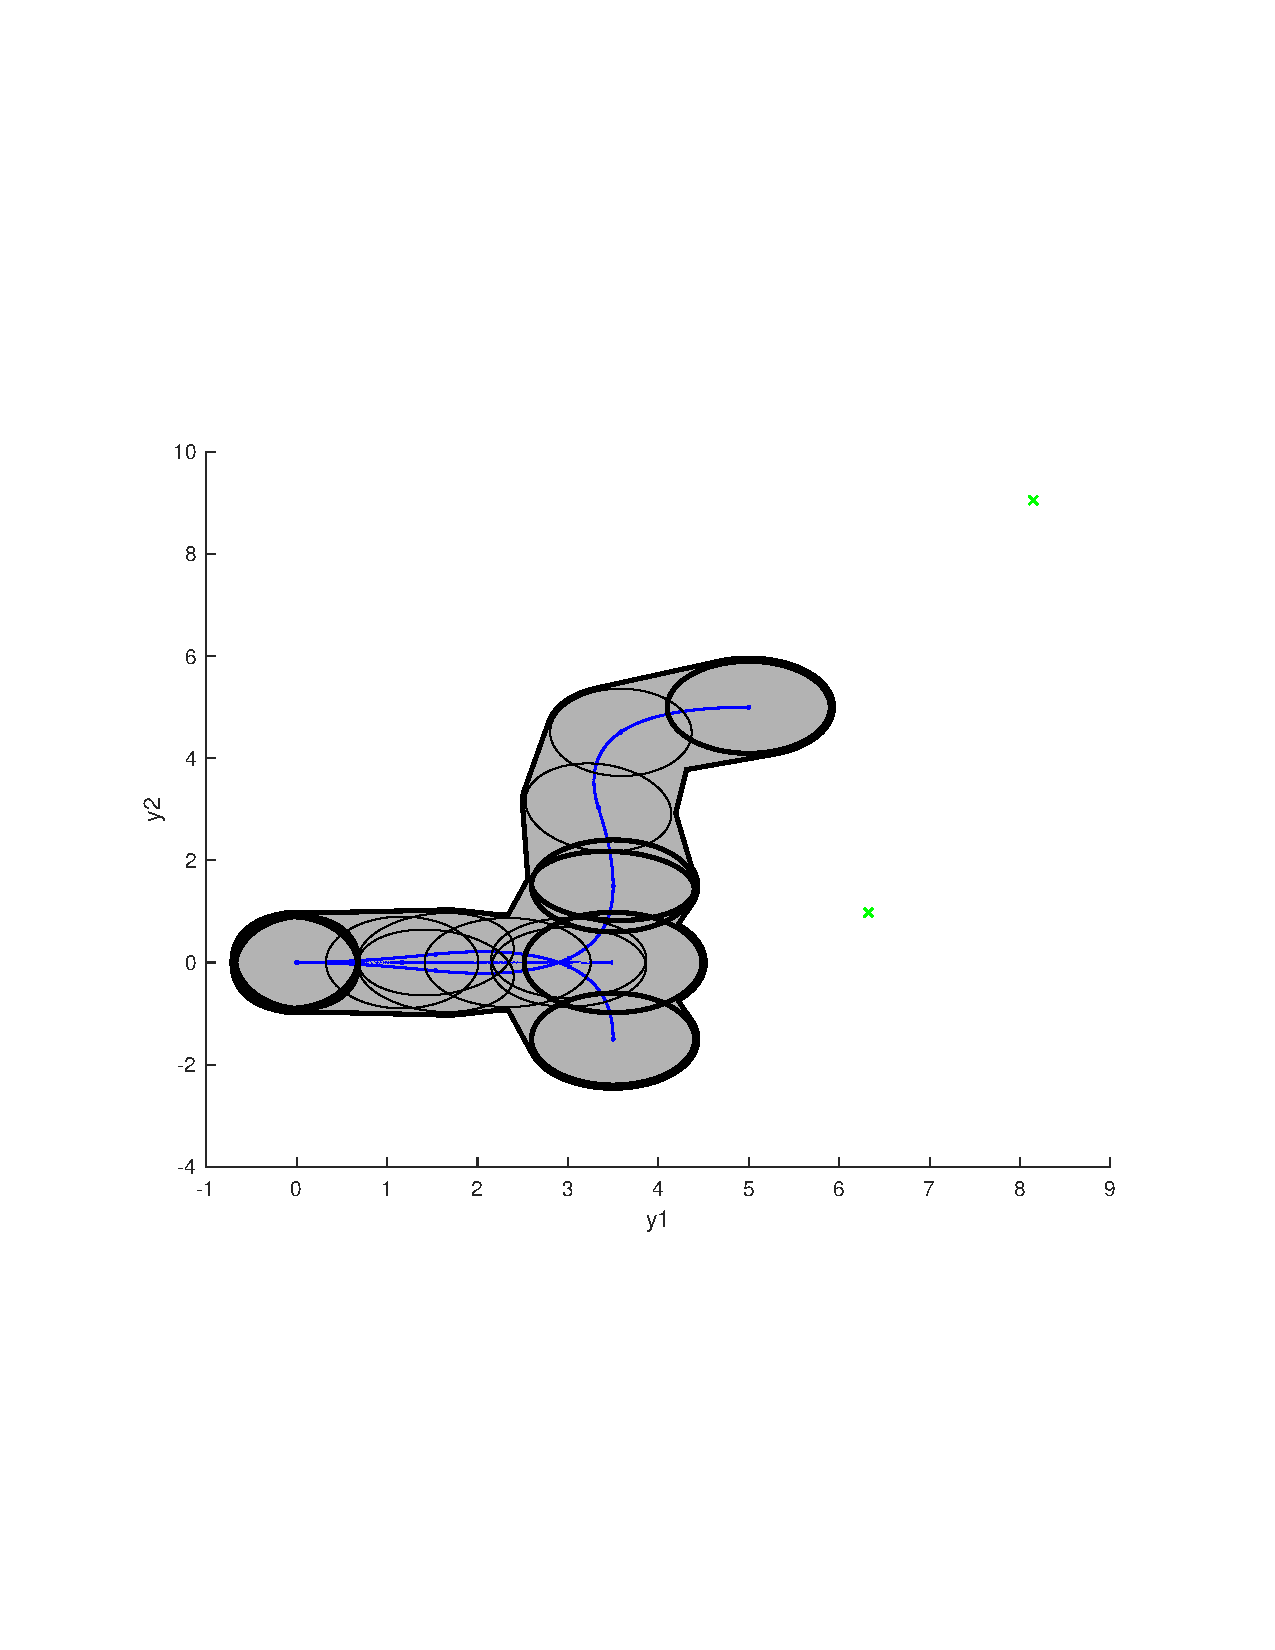
\includegraphics[scale=.5]{figures/rrtfunnel/euclidean-distance-closest-funnel3}
\caption{Another point picked uniformly from the state space.}
\end{figure}

\begin{figure}
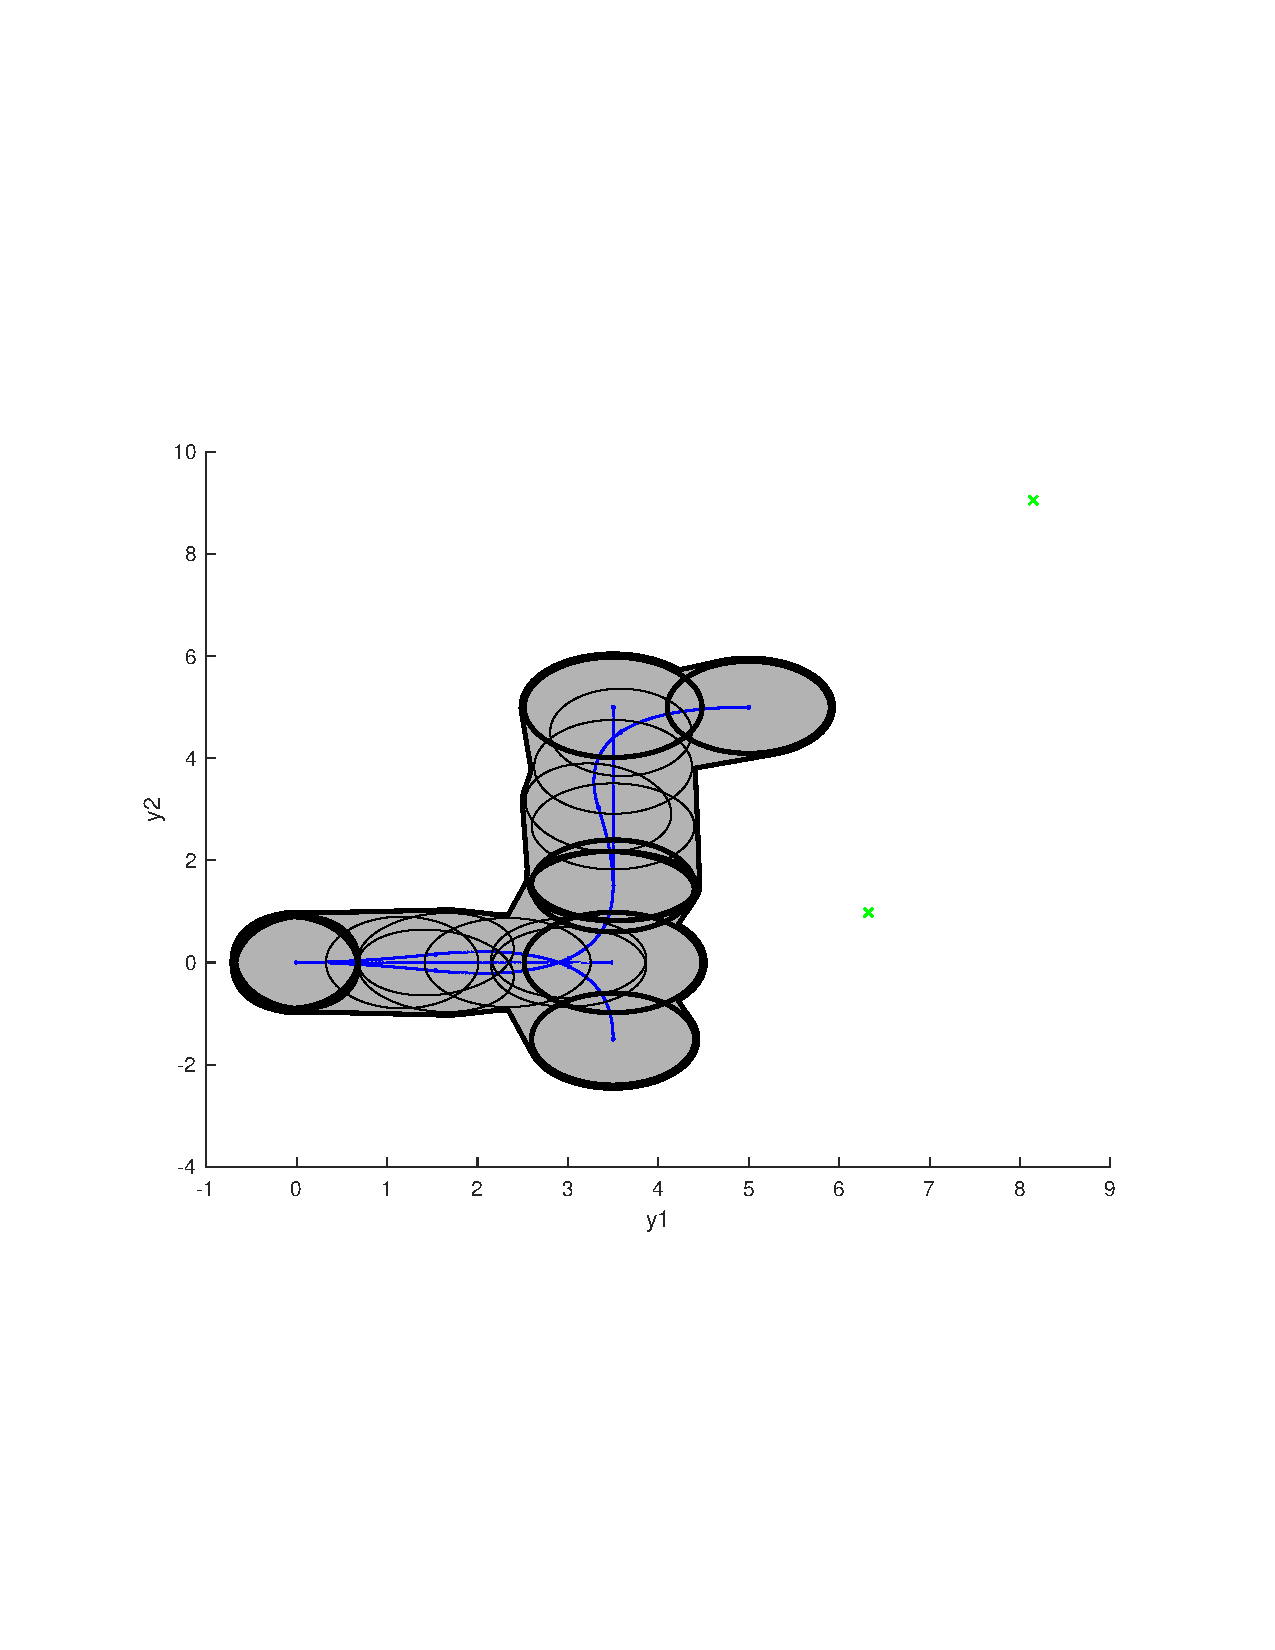
\includegraphics[scale=.5]{figures/rrtfunnel/euclidean-distance-closest-funnel4}
\caption{The funnel chosen by the local extension operator shows the limitations
of the Euclidean distance metric in the RRTFunnel algorithm.}
\end{figure}

This weakness is not unexpected if you take into consideration the non-holonomic
dynamics of our model vehicle.


\begin{figure}
  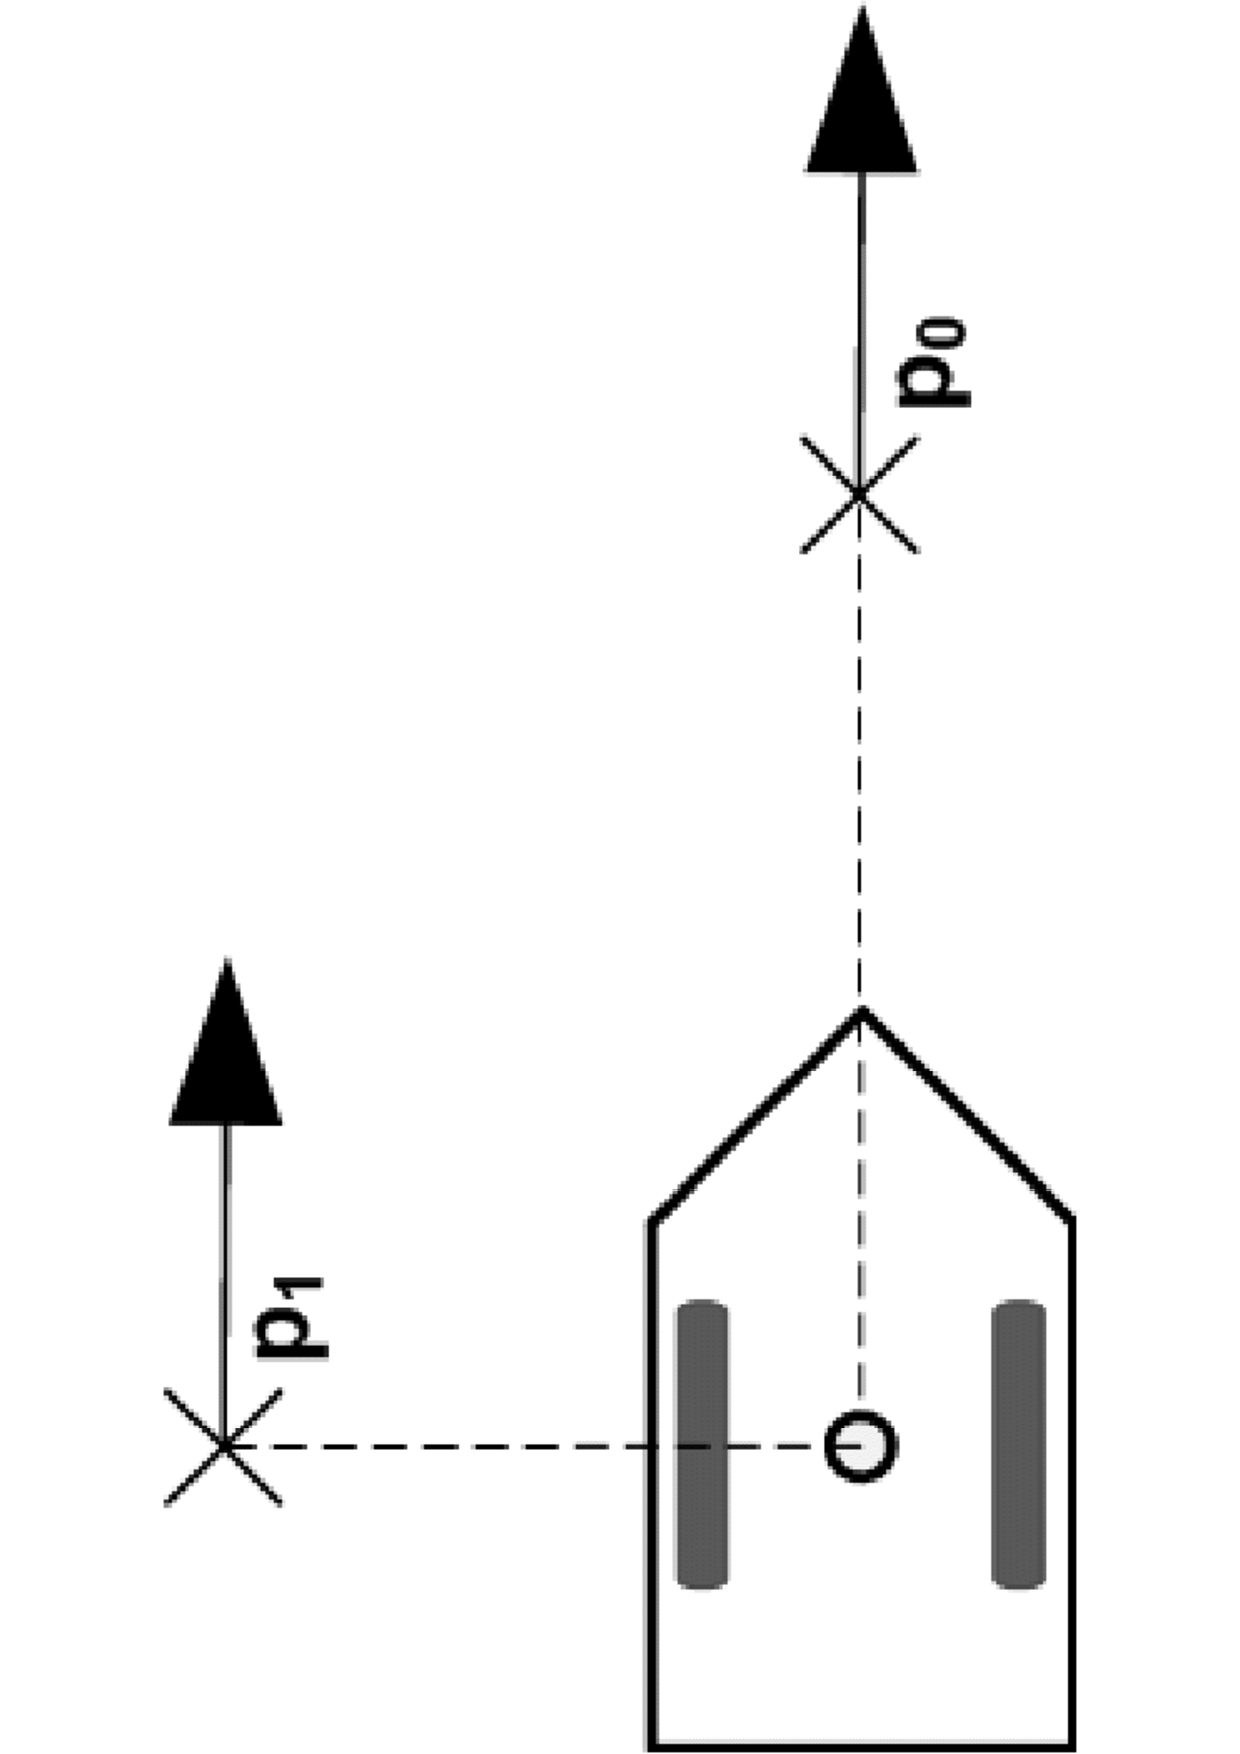
\includegraphics[scale=.3,angle=-90]{figures/rrtfunnel/non-holonomic-vehicle-euclidean-weakness}
  \caption{Consider two poses \(p_0\) and \(p_1\). Although \(p_1\) is nearer
    the robot in Euclidean distance it is harder to get to due to differential
    constraints. In this paper, we propose a directed distance function
    applicable to unicycle- type vehicles, that properly reflects the true
    cost-to-go of the system under the non-holonomic constraint. (figure
    courtesy of \cite{parkFeedbackMotionPlanning2015})}
\end{figure}

\subsection{Lyapunov function as a distance metric}

The weaknesses of the Euclidean distance metric lead to the discovery of the
\cite{parkFeedbackMotionPlanning2015} paper, in which the authors use the
\textit{Lyapunov function} as a distance metric for the extension operator in an
optimal \textit{RRT*} algorithm.

In \cite{SomePaperIHave}, blabla uses the lyapunov function as a distance metric
for the RRT algorithm. When this metric is applied to our RRTFunnel algorithm,
we get the following improvement upon the euclidean distance metric. Using the
same example as above:

% \begin{figure}
% \includegraphics{lyapunov-function-distance-closest-funnel}
% \end{figure}

% \begin{figure}
% \includegraphics{lyapunov-function-distance-extension-operator}
% \end{figure}